\documentclass[11pt,a4paper]{article}

\sloppy

\setlength{\textwidth}{16cm}
\setlength{\textheight}{23cm}
\addtolength{\hoffset}{-1.5cm}
\addtolength{\voffset}{-1.5cm}
\setlength{\headheight}{35pt}
\usepackage[utf8]{inputenc}
\usepackage[spanish]{babel}
\usepackage{ae}
\usepackage{graphicx}
\usepackage{subcaption}
\usepackage{tikz,pgfplots}
\usepackage{epsfig}
\usepackage{multicol, array}
\decimalpoint
\usepackage{amsmath,amssymb, amsthm}
\usepackage{sectsty}
\usepackage{listings}
\usepackage{Sweave}

\usepackage{hyperref}
\hypersetup{
    colorlinks=true,
    linkcolor=blue,
    filecolor=black,      
    urlcolor=blue,
    citecolor=blue,
    anchorcolor=black
}
 
\urlstyle{same}


\usepackage{fancyhdr}
%\allsectionsfont{\mdseries \raggedright}
\decimalpoint
\usepackage[T1]{fontenc}
\usepackage{textcomp}
%\usepackage[slantedGreek]{mathpazo} %% ver psnfss2e
%\usepackage{pifont}
%\usepackage{newcent}
\pagestyle{fancy}
\lhead{ 2021 - El Segundo Año de la Pandemia\\ Departamento de Física  -- U.N.S.L.\\Lic. en Física - Física Experimental I}
\rhead{
\includegraphics[width=1cm]{/home/juan/Documentos/Docencia/unsl.jpg}}
%\pagenumbering{arabic}
%\setcounter{page}{1}
\setlength{\parskip}{3mm}



\usepackage{hyperref}
\hypersetup{
    colorlinks=true,
    linkcolor=blue,
    filecolor=black,      
    urlcolor=blue,
    citecolor=black,
    	anchorcolor=black
}
 
\urlstyle{same}


\begin{document}


\vspace*{0.250cm}

\begin{center}
{\bf \large {Física Experimental I}} \linebreak



\bf{ Software N$^o$ 1: Introducción a R}\linebreak
 
\end{center}

\section*{Guión} \nonumber

En esta primera clase veremos algunas características del lenguaje de programación R, que es un lenguaje de alto nivel orientado a la estadística. Intentaremos familiarizarnos con las operaciones y el método de funcionamiento general, sin intentar recaer en particularidades, a fin de no perder el objetivo final de este curso: leer, analizar e interpretar datos de mediciones.

Para esta primera clase pasaremos revista a algunos tipos de variables (objetos, en general) típicas del lenguaje, y la forma de indexarlos. Veremos algunas operaciones entre variables y un puñado de funciones que, operando con las variables, realicen tareas de nuestro interés.

Analizaremos brevemente --tal vez demasiado-- la idea de algoritmo, intentando comprender cuál es el propósito de realizar uno, y los pasos a seguir. Finalmente daremos una mirada a tres casos específicos de algoritmo, que realizan diferentes tareas.

\bigskip

\section{Introducción}

R es un lenguaje de programación, que entra en la clasificación de \textit{software libre} (por intención manifiesta del autor del software, se puede distribuir libremente, modificar, copiar, etc.). Este lenguaje de programación está dedicado específicamente a estadística, motivo por el cual aprenderemos algunas funciones básicas en Física Experimental I y en Tratamiento de Datos Empíricos.

Basta agregar que R fue desarrollado inicialmente por Robert Gentleman y Ross Ihaka del Departamento de Estadística de la Universidad de Auckland en 1993, a partir de otro lenguaje anterior llamado S. Hoy en día R es ``uno de los lenguajes más utilizados en investigación por la comunidad estadística, siendo además muy popular en el campo de la minería de datos, la investigación biomédica, la bioinformática y las matemáticas financieras. A esto contribuye la posibilidad de cargar diferentes bibliotecas o paquetes con funcionalidades de cálculo o graficación''  \textbf{\cite{wikiR}}.

Para la ejecución de R, utilizaremos RStudio, que es un entorno gráfico que nos permite una utilización más cómoda del lenguaje de programación. RStudio es gratis en alguna de sus versiones, pero no es libre: nos contentamos, por ahora, con este entorno.

Agregaremos aquí algunas cuestiones que consideraremos importantes en este aprendizaje. La primera de ellas es una especie de axioma: \textit{la mejor forma de aprender a programar es...programando} (esta tonta tautología tal vez sea aplicable a casi cualquier disciplina en general). La segunda cuestión es que no hay que desesperar: gracias a internet, es posible encontrar una infinidad de foros de ayuda, de discusiones sobre cómo resolver un problema...lo cual facilita mucho las cosas\footnote{Los sitios de internet donde es posible encontrar códigos y preguntas son muchos, recomiendo dos:  R tiene su página oficial (\url{https://cran.r-project.org/manuals.html}); el segundo es StackOverflow, que es una página dedicada al intercambio de información sobre códigos -- se debe hacer un usuario para poder participar--, la dirección es \url{https://es.stackoverflow.com/} (en castellano), \url{https://stackoverflow.com/} (en inglés, con más documentos)}.

En general las personas se desaniman programando, a veces muy rápido. Aprender una lógica nueva es, a todas luces, un proceso engorroso. Para todos los estudiantes de este curso, diremos que no hay nada más útil (sin exagerar), ya que sólo un lenguaje de programación nos entrega la posibilidad de utilizar la computador como una \textit{máquina universal de Turing} (es decir, nos da toda la libertad posible en una computadora). La pista más seria para aprender (aunque pareciera zonzo) es ver un código hecho, y modificarlo...luego modificarlo otra vez....y otra vez...y otra vez...y así siguiendo hasta obtener...otro código. De antemano prevenimos, cualquiera puede programar, adquirir la lógica es una cuestión de tiempo.


\section{Primeros pasos}

La consola es la ventana ``activa'' de R. Puede funcionar como una calculadora. Pruebe sumando dos números cualesquiera, por ejemplo:

\begin{Schunk}
\begin{Sinput}
 2+3
\end{Sinput}
\begin{Soutput}
[1] 5
\end{Soutput}
\end{Schunk}

\noindent también podemos multiplicar dos números:
\begin{Schunk}
\begin{Sinput}
 2*3
\end{Sinput}
\begin{Soutput}
[1] 6
\end{Soutput}
\end{Schunk}

\noindent si nos interesa, podemos dividir dos números:

\begin{Schunk}
\begin{Sinput}
 2/3
\end{Sinput}
\begin{Soutput}
[1] 0.6666667
\end{Soutput}
\end{Schunk}

\noindent podemos preguntar si un número es igual a otro:

\begin{Schunk}
\begin{Sinput}
 2 == 3
\end{Sinput}
\begin{Soutput}
[1] FALSE
\end{Soutput}
\end{Schunk}

\noindent que es obvio que es falso (\texttt{FALSE})...sin embargo habitualmente se quieren realizar tareas más complejas que utilizar un lenguaje de programación en la forma que utilizamos una calculadora. Por lo que entraremos en los tipos de variables, para aprender algunos de los tipos más utilizados.



\section{Tipos de \textit{variables}}

En esta sección veremos algunos \textit{tipos de variables} que son de común utilización en R. Una variable en un lenguaje de programación es algo \textit{parecido} -pero no igual- a una variable en matemática. Es un espacio de memoria RAM (de tamaño no definido en este caso) con un nombre como ``etiqueta''.

En lenguajes orientados a objetos, como R, el nombre de ``variable'' es un poco  impreciso; el nombre correcto es \textit{objeto}. En R todo es un objeto, las funciones, las variables, las operaciones, etc...pero esto es un tecnicismo que no nos dirá nada, salvo que querramos bucear en la informática. Baste decir que no nos demoraremos en estas precisiones para meternos de lleno en su uso.

\subsection{Vectores Atómicos}

Probemos \textit{guardar} cinco números enteros en la \textit{variable} ``vector1'', escribiendo en la consola:

\begin{Schunk}
\begin{Sinput}
vector1 <- c(1,2,3,4,5)
\end{Sinput}
\end{Schunk}

\noindent en vez de usar el símbolo igual, en R es preferible escribir dos símbolos (\texttt{<-} ó \texttt{->}) que lo reemplazan,  simulando una flecha (también es posible escribir \texttt{c(1,2,3,4,5) -> vector1}). Por otra parte, la función \textbf{\textit{c()}} (concatenar) es muy usada, y sirve para crear listas de números (enteros, decimales y complejos), letras o caracteres lógicos. En este caso guardamos la concatenación de números en la variable ``vector1''. Para ver el contenido de la variable, podemos escribir el nombre de la misma en la consola y presionar \textit{ENTER}:

\begin{Schunk}
\begin{Sinput}
vector1
\end{Sinput}
\begin{Soutput}
[1] 1 2 3 4 5
\end{Soutput}
\end{Schunk}

\noindent como se puede ver, la \textit{variable} de R es una ``colección ordenada'' de números enteros (\textit{integer}). Existen otros tipos de variables, números con cifras decimales (``numeric''), letras (``character''), lógicas (``logic'', verdadero = TRUE, falso = FALSE). Este es el tipo de variable más simple en R, denominada \textit{vector atómico}. Para saber a qué clase corresponde, podemos escribir:

\begin{Schunk}
\begin{Sinput}
 class(vector1)
\end{Sinput}
\end{Schunk}
\noindent  esto nos da una idea de cómo operar con la variable en distintas operaciones, es decir, no es posible sumar caracteres, ni dividir variables lógicas (salvo coerción).

Por otra parte existe una medida especial de la cantidad de elementos contenidos en un vector atómico. Esto se denomina \textit{\textbf{length()}} (longitud, en inglés). Es claro que escribir:

\begin{Schunk}
\begin{Sinput}
length(vector1)
\end{Sinput}
\end{Schunk}
\noindent nos entrega el resultado de 5.

\subsubsection{Indexación de vectores atómicos}
Como los vectores atómicos de R son una lista ordenada, es posible obtener uno por uno los valores de la variable ``vector1'', escribiendo en la consola el nombre de la variable seguido de la posición que deseamos entre corchetes:
\begin{Schunk}
\begin{Sinput}
vector1[5]
\end{Sinput}
\begin{Soutput}
[1] 5
\end{Soutput}
\end{Schunk}

A la operación anterior la llamamos indexación, es decir, la utilización de un índice (en el caso anterior, 5) para llamar una porción de la variable vector1.

Otra forma de indexar consiste en \textit{llamar}  una porción mayor de la variable vector1, escribiendo entre los corchetes un \textit{intervalo}, denotado por dos números separados por ``\textbf{:}'':

\begin{Schunk}
\begin{Sinput}
vector1[1:3]
\end{Sinput}
\begin{Soutput}
[1] 1 2 3
\end{Soutput}
\end{Schunk}

Una tercera manera puede ser llamar los elementos de \textit{vector1} que sean \textit{menores o iguales} que 4, como mostramos a continuación:

\begin{Schunk}
\begin{Sinput}
vector1[vector1 <= 4]
\end{Sinput}
\begin{Soutput}
[1] 1 2 3 4
\end{Soutput}
\end{Schunk}

\noindent los símbolos de comparación nos entregan porciones de la variable vector1, indexada con \textit{una condición lógica}, es decir, indexamos usando una \textit{condición lógica}. Si miramos en detalle podemos ver que:

\begin{Schunk}
\begin{Sinput}
vector1 <= 4
\end{Sinput}
\begin{Soutput}
[1] TRUE TRUE TRUE TRUE FALSE
\end{Soutput}
\end{Schunk}

\noindent tenemos un vector cuyos elementos son las palabras reservadas TRUE y FALSE. A la hora de indexar esto se puede usar de la manera que se nos ocurra, y nos permite una buena plasticidad del lenguaje\footnote{Esto es particularmente cierto para cualquier lenguaje basado en objetos, como Python, R --que son muy parecidos--, Matlab, Julia, etc...}.



\subsubsection{Operaciones con vectores atómicos}

Podemos--obviamente-- realizar operaciones con la variable. Si la multiplicamos por un escalar, utilizando el símbolo ``*'', escribiendo:

\begin{Schunk}
\begin{Sinput}
vector1 * 2
\end{Sinput}
\begin{Soutput}
[1]  2  4  6  8 10
\end{Soutput}
\end{Schunk}

\noindent estamos multiplicando cada número de la variable por el escalar 2.

Ahora, para ver cómo operan las variables entre sí, creemos otra variable \textit{parecida} a ``vector1''- pero con los números al \textit{revés}, llamada vector2:
\begin{Schunk}
\begin{Sinput}
vector2 <- c(5:1)
\end{Sinput}
\begin{Soutput}
[1] 5 4 3 2 1
\end{Soutput}
\end{Schunk}

\noindent notamos que, en lugar de escribir todos los números, simplemente escribimos dentro de la función concatenar el número inicial y el final, separados por dos puntos.

Ahora intentemos sumar nuestros vectores entre sí (símbolo $\mathbf{+}$), y almacenar el resultado en una variable que llamaremos suma. Luego podemos multiplicarlos (símbolo \textbf{*}), almacenando el resultado en una variable llamada producto: ¿cómo R realiza las operaciones? Es fácil ver que las operaciones definidas en R se aplican, ordenadamente, en cada par de números, para dar otro vector atómico. En el caso de la suma, podríamos pensar que es análoga a la suma de vectores, de dimensión arbitraria (5 en este caso). En el caso del producto, nada tiene que ver con las operaciones que habitualmente están definidas en álgebra, ni el producto escalar entre vectores, ni el producto vectorial se asemejan a la operación hecha por R.

Por otra parte, podremos definir una tercera variable:
\begin{Schunk}
\begin{Sinput}
vcorto <- c(1,2)
\end{Sinput}
\begin{Soutput}
[1] 1 2
\end{Soutput}
\end{Schunk}

\noindent  miremos el resultado de las operaciones introduciendo el nombre de la variable. Ahora multipliquemos \texttt{vcorto*vector1} . ¿Cómo realiza la operación R? Es posible ver que la variable más corta se repite cuantas veces sea necesario, de manera ordenada, para operar con la variable más ``larga''. En este caso particular, \texttt{vector1} tiene 5 números, mientras que \texttt{vcorto} tiene dos. Es por eso que R nos avisa que \texttt{vcorto} se ha repetido un número no entero de veces, i.e. la \textit{longitud} del objeto mayor no es múltiplo entero de la longitud del objeto menor. A estos avisos se los denomina \texttt{\textbf{warnings}} (advertencias, en inglés), y nos dicen cuándo puede haber problemas, sin detener la ejecución de la operación. Cuando hay un \texttt{\textbf{error}}, R detiene la ejecución de la operación.


\subsection{Matrices}

Las matrices en R son idénticas a las del álgebra: un arreglo de números en filas y columnas. Para escribir una matriz, deberemos escribir los elementos y el número de filas (nrow) y columnas (ncol):

\begin{Schunk}
\begin{Sinput}
M <- matrix(c(1:9), nrow=3, ncol=3)
\end{Sinput}
\begin{Soutput}
       [,1] [,2] [,3]
[1,]    1    4    7
[2,]    2    5    8
[3,]    3    6    9
\end{Soutput}
\end{Schunk}

Lo anterior hace una matriz de $3\times 3$. Para ver la variable, escribimos el nombre y presionamos ENTER. Antes de seguir, charlaremos un poco de cómo indexar las matrices y cómo llenarlas, es decir, cuestiones importantes referidas a objetos de dimensiones $n \; \times \;m$.


\noindent hacemos notar algunas cosas de la matriz M que acabamos de escribir:


\begin{itemize}

\item[$\bullet$] \textbf{Indexación de matrices:} aparecen números entre corchetes (a la izq. y arriba en la matriz), que nos indican los índices. Estos números pueden servir para llamar elementos específicos de la matriz. Por ejemplo, si queremos obtener el elemento de la segunda fila y la tercera columna, escribiremos $M[2,3]$ (las filas primero, las columnas segundo); para llamar \textit{todos} los elementos de una fila, dejamos vacío el número de columna (para la primera fila podemos escribir \texttt{M[1,]}); al contrario hacemos con las columnas, deberemos hacer \texttt{M[,2]} para obtener los elementos de la segunda columna (dejar el espacio vacío significa que seleccionamos \textit{todos} los elementos, tanto de filas como columnas).

\item[$\bullet$] El orden de entrada de los números, tal como está escrito el comando, por defecto se indica que la matriz \texttt{M} se llena por columnas (i.e., se llena la primera columna, luego la segunda, etc.). Podemos cambiar esto -llenarlo por filas- si escribimos:

\begin{Schunk}
\begin{Sinput}
 M <- matrix(c(1:9), nrow=3, ncol=3, byrow = T)
\end{Sinput}
\begin{Soutput}
     [,1] [,2] [,3]
[1,]    1    2    3
[2,]    4    5    6
[3,]    7    8    9
\end{Soutput}
\end{Schunk}

\noindent notemos que la opción \texttt{\textbf{byrow = T}} (que en inglés es \textit{por filas}), en la función \texttt{matrix()}, es declarada como \texttt{TRUE (T)} (verdadera). Esto hace que el resultado de la operación no sea el mismo.
\end{itemize}

Las operaciones de sumar, restar, multiplicar, dividir, etc. se realizan de la misma manera que con los vectores, i.e., las operaciones se realizan entre pares de elementos con el \textit{mismo} índice. Podríamos probar multiplicando dos matrices pequeñas.

Por último, para saber la cantidad de columnas en la matriz \texttt{M}, podemos escribir ``\texttt{ncol(M)}''. Para el número de filas, ``\texttt{nrow(M)}''. Para el número de filas y el de columnas, ``\texttt{dim(M)}'', lo que nos entrega un vector con dos elementos que son el número de filas y de columnas.

\subsection{Data Frames}

Si bien R maneja muchos tipos de variables, los \textit{dataframes} son la forma de almacenar datos más ``amena'' de este lenguaje. Un \textit{data frame} (una traducción posible sería ``marco de datos'') es un arreglo de números del mismo estilo que una matriz. Sin embargo posee algunas características distintivas:

\begin{itemize}
\item[$\bullet$] Las columnas pueden poseer tipos diferentes de variables (por ejemplo, la primera columna puede estar compuesta por caracteres, la segunda por números, etc...).

\item[$\bullet$] Cada columna puede poseer un nombre, lo que hace más fácil el manejo de datos, aunque también podemos indexar, como en las matrices o en los vectores atómicos, utilizando números entre corchetes. 
\end{itemize}

Para crear un \textit{dataframe} pequeño, nos proponemos hacer una tabla que contenga nuestros nombres en una columna, nuestra edad en otra columna, y la cantidad de hijos que tenemos en una tercer columna (podemos obviar o falsear datos, ¡no es necesario decir la verdad!). Como primer paso, creamos un vector atómico de nombres. Para esto, escribiremos nuestros nombres completos utilizando la función concatenar y los asignaremos al vector atómico \textit{nombre}. Recordemos que cada nombre debe ir entre comillas y que debemos separar entre nombres con comas, como se muestra a continuación:
\begin{Schunk}
\begin{Sinput}
> nombre <- c("Juan Pablo de Rosas"', "Ricardo Rubén", "Roberto Carlos")
\end{Sinput}
\end{Schunk}

Luego creamos el vector atómico ``edad'': \texttt{ edad <- c(35, 25 ,76)}

Y, por último, creamos el vector conteniendo la cantidad de hijos (yo no tengo, Ricardo Rubén no sabemos y Roberto Carlos tiene cuatro), lo que nos deja: \texttt{ hijos <- c(0,NA,4)}.

con estos vectores, utilizamos un comando muy simple, para crear el \textit{dataframe} tabla:

\texttt{>tabla <- data.frame(nombre,edad,hijos)}\footnote{Es \textit{una} de varias formas de crear \textit{dataframes}...el resto irá apareciendo en la práctica. Por otra parte, lo habitual es \textit{cargar} un \textit{dataframe} de un archivo de texto, de una imagen, o de una fuente de datos. La forma utilizada aquí es por demás engorrosa, pero sirve como ilustración.}

Con los datos cargados en la variable \textit{tabla}, notamos algunas particularidades:

\begin{itemize}
\item[$\bullet$] Cada columna tiene su nombre, aunque están ordenadas también numéricamente. Con esto podemos seleccionar la primer columna de dos maneras. La primera de ellas es la misma que una matriz, escribiendo ``\texttt{> tabla[ ,1]}''. La segunda de ellas es más simple y manejable, podemos escribir \texttt{>  tabla\$nombre}.

\item[$\bullet$] Para saber los nombres de las columnas de un \textit{dataframe} podemos utilizar ``\texttt{ colnames(tabla)}'' (esto nos arroja un vector con los nombres de las columnas). También es posible cambiar los nombres de las columnas utilizando la misma función, aunque de manera diferente:
\begin{Schunk}
\begin{Sinput}
colnames(tabla) <- c('columna1', 'columna2', 'columna3')
\end{Sinput}
\end{Schunk}

\item[$\bullet$] Una forma de indexación útil, también, puede ser una \textit{condición lógica}. Por ejemplo, si quisiera saber cuál es la información de ``Roberto Carlos'' (seleccionar la fila de datos sobre Roberto Carlos), podríamos escribir:
\begin{Schunk}
\begin{Sinput}
tabla[tabla\$nombre == "Roberto Carlos",]
\end{Sinput}
\end{Schunk}


$\begin{matrix}

 & nombre & edad & hijos \\
2 & Roberto\hspace{0.1cm} Carlos &  76  &  4

\end{matrix}$

\noindent este comando puede no resultar de mucha utilidad aquí, en un \textit{dataframe} que tiene tres filas. Sin embargo si se trata de un set de datos muy grande, este tipo de indexación nos servirá de mucho\footnote{Aunque aclaramos que \textit{indexar} por medio de caracteres es una operación realmente lenta para una computadora, cuyo tiempo de cómputo crece con el cuadrado del largo de vector...algún día pensaremos por qué.}.
\end{itemize}

\subsection{Valores especiales}

Si bien, en principio, es posible utilizar cualquier nombre para una variable, hay combinaciones de caracteres especiales, que refieren a funciones o a \textit{palabras reservadas} por el lenguaje para funciones específicas. Algunas de ellas son:

\begin{itemize}
\item[$\bullet$] Las constantes lógicas \texttt{TRUE} (verdadero) y \texttt{FALSE} (falso) son palabras reservadas porque se utilizan para operaciones lógicas. También pueden ser reemplazadas por la primera letra, \texttt{T} ó \texttt{F}, las cuales están reservadas igualmente.

\item[$\bullet$] \texttt{NA} es una combinación de caracteres bastante común en R. Quiere decir \texttt{N}ot \texttt{A}vailable (No Disponible, en inglés), y se utiliza mucho en estadística, indicando la imposibilidad de completar un dato en una lista. Es una constante lógica (en R, no en el álgebra booleana).

\item[$\bullet$] \texttt{Inf} es el símbolo para indicar Infinito. Esto tiene semejanzas con la matemática, pero en un lenguaje de estas características se obtiene como resultado de ``saturar'' la cantidad de números posibles en la computadora. Lo obtendremos al realizar operaciones como \texttt{1/0}; también obtendremos \texttt{-Inf} como resultado de \texttt{-1/0}, aunque también en sumas de enteros muy grandes.
 
\item[$\bullet$] \texttt{NaN} es \textbf{N}ot \textbf{a} \textbf{N}umber (No un Número, en inglés), y se obtiene típicamente de realizar operaciones inválidas, como por ejemplo cualquiera que involucre infinito: \texttt{Inf*0}, \texttt{Inf/Inf}, etc..
\end{itemize}


\section{Otras operaciones}

Siendo R un lenguaje orientado a la estadística, posee algunos comandos que nos serán de utilidad. Enumeramos algunos:
\begin{itemize}

\item[$\bullet$] El comando \texttt{mean()} (media en inglés). Es, simplemente, lo que se conoce popularmente como el promedio. Para verlo, podemos sacer la edad \textit{media} de todos los que estén en la lista de la variable tabla\$edad, escribiendo \texttt{mean(tabla\$edad)}. El resultado de la operación es la suma de todos los valores de la variable, dividido la cantidad de personas en la lista total.

\item[$\bullet$] Otra operación muy usada es \texttt{sum()}, la cual suma todos los elementos del la variable que esté entre paréntesis. Probemos escribiendo \texttt{sum(tabla\$edad)}. Divida el resultado por la cantidad de personas. ¿Muestra alguna relación con \texttt{mean(edad)}?.


\end{itemize}

\textbf{Tarea1}

\begin{itemize}

\item[1.a] Calcule la suma de edades de todos los miembros del grupo, en la variable \textit{tabla}. Para esto, puede utilizar el comando ``\texttt{> sum(tabla\$edad)}'' (suma todos los valores de la columna edad de la variable tabla).

\item[1.b] Calcule la edad media del grupo. Para esto debe hacer el cociente entre la suma de todas las edades y la cantidad de edades que sumó...compárelo con \texttt{mean(tabla\$edad)}

\item[1.c] Calcule la cantidad media de hijos de los sujetos de la variable \texttt{tabla}...

\end{itemize}


\section{Algoritmos (una vaguísima noción)}

El concepto de \textit{algoritmo} no está definido de manera consensuada. Sin embargo es una palabra que cada vez adquiere más popularidad debido a la creciente influencia de los procesos automatizados en la vida cotidiana. La palabra algoritmo es debida a un prominente matemático árabe, por lo tanto no es imposible pensar que este concepto esté relacionado de alguna forma con el mundo de los números.

Procediendo, tal vez torpemente, le robamos a la famosa Enciclop\ae dia Britannica\footnote{Traducido para usted desde \url{https://www.britannica.com/science/algorithm}}:

``Un \textit{algoritmo} es una conjunto sistemático de procedimientos --en un número finito de pasos-- que responden a una pregunta  o solucionan un problema. El nombre deriva de la publicación latina \textit{Algoritmi de numero Indorum}, (``al-Khwuarizmi: Sobre el arte hindú para calcular'') que es una traducción del libro escrito por el matemático musulmán del S. IX  al-Khwarizmi \footnote{Abu Abdallah Muhammad ibn Musa al-Jwarizmi (Abu Yaffar), conocido generalmente como al - Juarizmi, fue un matemático, astrónomo y geógrafo persa musulmán, que vivió aproximadamente entre los entre los años 780 y 850 de nuestra era. El nombre del libro \textit{Algoritmi de numero Indorum} es la traducción latina, a la cual le agregaron el nombre \textit{latinizado} del autor. La versión original del nombre del libro, en árabe, tiene la palabra \textit{al-jabr}, que dio nombre a la rama de las matemáticas conocida como álgebra...así de importante fue este notable matemático.}.

Podemos agregar que un algoritmo permite realizar una actividad mediante pasos sucesivos que no generen dudas a quien deba realizar dicha actividad \footnote{Wikipedia en español.}. Esta definición es bastante agradable: podemos pensar desde una receta de cocina, una partitura de música o las reglas de derivación como ejemplos...y también un código de R.


\section{Y... ¿Qué sería un algoritmo en R?}

Una de las grandes ventajas de programar es que tenemos a mano la posibilidad de \textit{escribir un código} (hacer un algoritmo) que cargue y levante datos de manera automática, para el fin que deseemos.

En el caso que nos compete, la programación estadística en R, es claro que \textbf{no} vamos a estar utilizando la consola todo el tiempo, sino que sería muy agradable escribir una serie de instrucciones que, operando sobre datos de entrada, nos entreguen por salida los resultados que necesitemos. La idea es que cada línea del archivo de texto debe incluir una instrucción (como si la estuviéramos escribiendo en la consola). Las instrucciones se van ejecutando una a una, de manera secuencial (una por vez, de manera ordenada).

Para hacer un algoritmo en R es necesario generar un archivo de texto (generalmente es de extensión *.R), conteniendo líneas de \textit{código} (instrucciones del lenguaje). Luego utilizando el botón ``Source'', R ejecutará secuencialmente (de la primera a la última) nuestro código. Cada línea debe estar libre de errores de redacción (no se va a interpretar nada que esté mal escrito), por lo que puede resultar una tarea, al principio, muy engorrosa. Para ejecutar una línea o una parte de un código, es posible: a) seleccionar una parte del código y presionar el botón \textit{Run}, al lado de \textit{Source} b) poner el cursor en una línea y apretar \texttt{Ctrl + ENTER}. Ejecutar pedazos o líneas de un código es importante para hacer \textit{debugging} (desenbichado, en inglés), es decir, en criollo, encontrar los posibles errores del código.

Un algoritmo es escrito y reescrito muchas veces antes de tener una versión final. Esto no quiere decir que debamos bajar los brazos de antemano, sino que constituye una advertencia para aquellos de nosotros que tengamos una predisposición natural a querer resultados rápido: cuesta aprender a escribir algoritmos, como cuesta aprender cualquier otra cosa. La ganancia es que, una vez listos, los algoritmos pueden ser alimentados una y otra vez con diferentes datos, lo que ahorra una cantidad considerable de trabajo que hasta hace no mucho tiempo debía hacerse una y otra vez a mano o con la ayuda de máquinas de cálculo.

A continuación, tres ejemplos de algoritmos que servirán para aclarar un poco el panorama.


\subsection{Un curso de estudiantes...}

Como ejemplo proponemos un conjunto de notas de un grupo de 30 estudiantes. Queremos obtener ciertos  parámetros relacionados a las notas obtenidas por el curso, un gráfico de distribución de las notas, la media, etc. Un algoritmo que implementa estas cosas se muestra en la página siguiente. Aclaramos dos cosas antes de empezar:

\begin{itemize}
\item[$\bullet$] El símbolo ``\texttt{\#}'' sirve para \textit{comentar}, es decir, para agregar líneas explicativas de código que R \textit{no interpreta}. Esto es muy útil para recordar cómo y para qué funciona un código después de algunos meses sin usarlo.
\item[$\bullet$] El ingreso de los datos no es representativo. Habitualmente cargamos a partir de un archivo de texto o de Excel los conjuntos de datos. Acá lo hacemos así para ahorrarnos un tiempo.
\item[$\bullet$] En general los códigos comienzan por limpiar la memoria del entorno de lenguaje (Global Environment en este caso). Esas son las líneas \textit{extrañas} al comienzo del código. Sirven para que el código no utilize datos de una corrida anterior.
\end{itemize}
\pagebreak

\begin{Schunk}
\begin{Sinput}
#Limpieza de entorno. Aca aparecen unos comandos extragnos...que borran todo
#Borra consola, variables y funciones definidas en el entorno Global
rm(list = setdiff(ls(), lsf.str()));
rm(list=lsf.str());
cat("\014")


#(aca escribimos todo sin acentos...)

#PRIMER PASO
#Cargamos las notas de los 30 estudiantes
#De paso: una forma de no alargar demasiado cada
#linea, usando un simbolo "+"
notas <- c(3.1, 4.6, 2.7, 3.6, 3.6, 1.7, 3.8, +
             4.9, 4.1, 2.3, 1.6, 2.9, 4.1, 2.6, + 
             4.2, 7.5, 7.0, 8.3, 9.0, 7.9, 8.2, 8.6, + 
             7.9, 7.5, 8.2, 7.9, 8.1, 8.1, 9.5, 10)


#Nos fijamos si la cantidad de numeros que metimos es 30
show( length(notas) )

#Calculamos la media (el promedio) del curso
media <-  mean(notas) 

#Calculamos la mediana de las notas
mediana <- median(notas)

#Vemos el rango de la variable notas (la menor y la mayor)
rango <-  range(notas)


#vemos la dispersion de datos mediante un histograma
show( hist(notas, breaks = 10, probability = T))
#notamos que parece haber dos modas

#graficamos la densidad de prob con el kernel
#y notamos que tiene dos maximos...
lines(density(c(notas,10)), lwd = 2, col = "red")

sprintf('La media de las notas es: %f \n', media)
sprintf('La mediana de las notas es: %f \n', mediana)
sprintf('El rango de las notas es: %f \n', rango[2]-rango[1])
sprintf('La nota minima es: %f \n', rango[1])
sprintf('La nota maxima es: %f \n', rango[2])
\end{Sinput}
\end{Schunk}

\pagebreak


\subsection{Producto Escalar...}
Como vimos en el código anterior, podemos sacar algunos resultados útiles a partir de un código simple, aunque es verdad que lo anterior lo podríamos haber hecho con Excel o cualquier otro software. Está bien para empezar, pero hasta aquí no un lenguaje no muestra ninguna virtud respecto de sus competidores con entorno gráfico...es sólo para entrenar.

Si bien en R las variables son \textit{vectores}, ya vimos que éstas no se multiplican según las reglas del producto escalar del álgebra. Vamos a hacer un algoritmo que calcule un producto escalar y nos diga el ángulo entre dos vectores cualesquiera en 2D.

Para aquellos que no se acuerdan del producto escalar, una pequeña definición:

Sean los vectores $\vec{\mathbf{v_1}}$ y $\vec{\mathbf{v_2}}$( $\in \, V^2$), separados por un ángulo $\theta$:

\begin{eqnarray}
\vec{\mathbf{v_1}} &= x_1 \hat{\mathbf{\imath}} + y_1 \hat{\mathbf{\jmath}} \\
\vec{\mathbf{v_2}} &= x_2 \hat{\mathbf{\imath}} + y_2 \hat{\mathbf{\jmath}}
\end{eqnarray}

El producto escalar $\vec{v_1}\cdot \vec{v_2}$ estará dado por:
\begin{eqnarray}
\label{1}\vec{\mathbf{v_1}} \cdot \vec{\mathbf{v_2}} &=& (x_1 \hat{\mathbf{\imath}} + y_1 \hat{\mathbf{\jmath}}) \cdot (x_2 \hat{\mathbf{\imath}} + y_2) \hat{\mathbf{\jmath}}  \\
\label{def} \vec{\mathbf{v_1}} \cdot \vec{\mathbf{v_2}} &=& x_1 x_2 + y_1 y_2 \\
\label{3} \vec{\mathbf{v_1}} \cdot \vec{\mathbf{v_2}} &=& \mid \vec{\mathbf{v_1}} \mid \hspace{0.1cm} \mid \vec{\mathbf{v_2}} \mid cos(\theta) \Rightarrow \\
\label{cos} cos(\theta) &=& \dfrac{\vec{\mathbf{v_1}} \cdot \vec{\mathbf{v_2}}}{\mid \vec{\mathbf{v_1}} \mid \hspace{0.1cm} \mid \vec{\mathbf{v_2}} \mid}  
\end{eqnarray}

\noindent del conjunto de ecuaciones, las que nos servirán son: la ec.(\ref{def}), que es una definición en función de las coordenadas cartesianas, y la ec.(\ref{cos}), que es lo que nos entrega el coseno del ángulo en función del producto escalar y los módulos de los vectores.

\begin{figure}[h!] 
\begin{center}
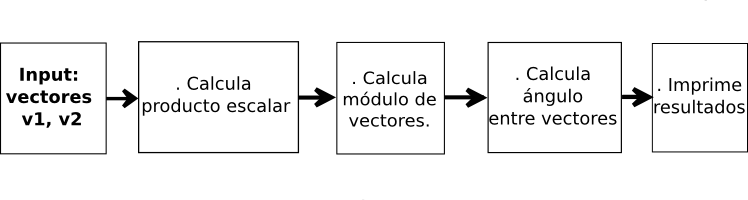
\includegraphics[width=0.8\textwidth]{pescalar.png}
\caption{Diagrama de flujos del código ``\texttt{prodescalar.R}''.}
\label{df}
\end{center}
\end{figure}

El código que hace todo esto es \href{http://linux1.unsl.edu.ar/~mdolz/Experimental_I_2do_cuatrimestre/Programacion_R/}{prodescalar.R}. Un diagrama de flujos\footnote{Un diagrama de flujos es un \textit{esquema} de bloques de lo que hace un código. Posibilita la visualización de operaciones de código complejos sin necesidad de \textit{entrar en detalle}.} de este código puede ser visto en la Fig.(\ref{df}), donde haremos notar que todo empieza en el \textit{input} del programa, que son los vectores. Luego se calculan las cantidades requeridas y finalmente se muestran los resultados por medio de un gráfico y algunas líneas de texto. No es para nada necesario que la \textbf{salida} ó \textbf{output} de este código finalice con las líneas de texto, sino que lo mostramos así para que no parezca tan \textit{árido}...con saber sólo en qué variables están los resultados necesarios, alcanza.


Daremos alguna mirada, cambiaremos los vectores de entrada, y ya está. Es importante prestar atención a cómo las ecs.(\ref{1}, \ref{def}, \ref{3} y \ref{cos}) son \textit{pasadas} al código\footnote{Hay lenguajes que son particularmente propicios para usar expresiones matemáticas \textit{parecidas} a las que escribimos con papel...Julia, Mathematica...no R, ni Python, ni C. Tendremos que acostumbrarnos.}. Este código no hace nada raro, pero muestra un poco cómo pasar desde \textit{el papel} a \textit{la pantalla}.

 \subsection{Estimando superficies}

Como tercer ejemplo de código, bajamos los archivos:
\begin{itemize}
\item[$\bullet$] \href{http://linux1.unsl.edu.ar/~mdolz/Experimental_I_2do_cuatrimestre/Programacion_R/}{supmano.R} \item[$\bullet$] \href{http://linux1.unsl.edu.ar/~mdolz/Experimental_I_2do_cuatrimestre/Programacion_R/}{mano.jpg}
\end{itemize}

A los archivos bajados los pondremos en el directorio en el que querramos trabajar. Luego, abramos el archivo \texttt{supmano.R}. En las primeras líneas de código vemos que hay una instrucción llamada \texttt{setwd()} (en inglés, acrónimo de \textbf{set} \textbf{w}orking \textbf{d}irectory) que es el directorio en donde R leerá los archivos\footnote{Esto se realiza con barras \textit{normales} (``/'') tanto en Linux como en Windows. Un ejemplo en Linux: \texttt{setwd(`/home/RicardoFort/Escritorio/')}; en Windows: \texttt{setwd(`C:/Users/JudithButler/Documents/')}}. Escriba la instrucción en donde haya colocado los archivos.

Como algunos de ustedes sabrán, las fotografías digitales no son otra cosa que arreglos numéricos en forma matricial. En nuestro caso, \texttt{mano.jpg}, es un archivo en escala de grises, por lo que tendremos una matriz que posee, en cada posición, un número entre $0$ (totalmente negro) y $1$ (totalmente blanco). Cada uno de los números es un \textit{píxel}, es decir, un \textit{cuadradito} de colores que pueden variar continuamente (...) entre el negro y el blanco.

\begin{figure}[h!]
\begin{subfigure}{.50\textwidth}
  \centering
  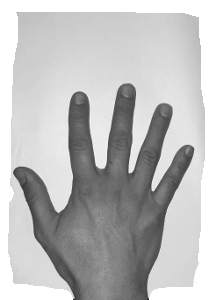
\includegraphics[width=1\linewidth]{manoorig.jpg}
  \caption{}
  \label{mano}
\end{subfigure}%
\begin{subfigure}{.50\textwidth}
  \centering
  
\includegraphics[width=1\linewidth]{manocont.jpg}
  \caption{}
  \label{manocon}
\end{subfigure}
\caption{Fotografía presente en \texttt{mano.jpg}, \textbf{(a)} antes de elegir un contraste \textbf{(b)} puntos seleccionados por contraste.}
\label{}
\end{figure}

Como introducción a este código simple, vamos a intentar estimar la superficie de la mano, \textit{indexando} mediante una \textit{condición} a la matriz de la imagen \texttt{mano.jpg}, a fin de contarlos. La condición que usaremos para la indexación será un contraste, es decir, un valor que intente definir la zona de la mano en la Fig.(\ref{mano}). El resultado de esta operación puede verse en la Fig.(\ref{manocon}). 

Una vez contados los píxeles de la mano, sólo nos resta saber que la superficie de la foto (que fue previamente recortada) es la de una hoja A4 --que tiene tamaño conocido, $29.7 \times 21 cm$-- que será usado para la calibración en unidades del Sistema Internacional.

La imagen presente en \texttt{mano.jpg} puede observarse en la Fig.(\ref{mano}). Puede ser cargada en R mediante una librería especial, que se instala sóla al correr el código. 


\textbf{Tarea en clase o casa:} Realizar un diagrama de flujos del código de esta sección.

\pagebreak

Las cuentas que nos permiten sacar la superficie de la mano son (un par de reglas de tres):
\begin{itemize}
\item[$\bullet$] La imagen tiene $i \times j$ píxeles.
\item[$\bullet$] La imagen tiene una superficie de $29.7cm \times 21cm = 623.7 cm^2$
\item[$\bullet$] La mano ocupa $m$ píxeles.
\item[$\bullet$] Entonces podemos calcular la superficie de la mano en $cm^2$ como $\dfrac{m}{i \times j} 623.7$
\end{itemize} 


Corramos el código, juguemos un poco con los parámetros, esta clase \textit{ha termináo'} (acostumbrándonos al gauchesco).

\section*{Resumen}
En esta clase vimos una pequeña introducción a R, visitando algunos tipos de objetos (vectores, matrices, \textit{dataframes}) y formas de extractar partes de cada objeto de distintas maneras: seleccionando índices, intervalos de índices y mediante la utilización de condiciones lógicas. 

Luego vimos una pequeña noción de algoritmo y algunas implementaciones un poco inútiles que esperamos que hayan servido para algo. La estadística de los estudiantes es un ejemplo aburrido, pero instructivo, de cómo se ve un código. El código que calcula cantidades de vectores es lo más aburrido que hay y no lo vamos a ver más, así es que a no preocuparse. Por último, \texttt{supmano.R} calculó la superficie de la mano de cierto individuo (humano, demasiado humano), utilizando una técnica simple. Este último código tal vez lo volvamos a ver...

Esta clase buscó mostrar ciertos comandos básicos, la forma de indexar objetos de R, y alguna muestra de cómo sacar provecho de algo a primera vista tan poco útil como es escribir códigos. Esperamos convencer a los estudiantes de que no es una actividad tan poco relacionada con este curso en la próxima clase.

La semana que viene continuaremos con algunas nociones de R que manejarán otros tópicos: Carga de datos, gráficos y un poquito de semiología de gráficos para finalmente caer en una de las prácticas más habituales en la experimentación, el ajuste lineal... 
\begin{thebibliography}{99}

\bibitem{wikiR} Wikipedia. \textit{https://es.wikipedia.org/wiki/R\_(lenguaje\_de\_programación)}.

\bibitem{wikial} Wikipedia. \textit{https://es.wikipedia.org/wiki/Algoritmo}

\end{thebibliography}.
\end{document}